\documentclass[landscape]{slides}
\usepackage[landscape, margin=2cm]{geometry}
\usepackage{color}
\usepackage{bm}
\usepackage{graphicx}
\usepackage{hyperref}
\usepackage{listings}
\definecolor{mygreen}{rgb}{0,0.6,0}
\definecolor{mymauve}{rgb}{0.58,0,0.82}
\lstset{ %
  backgroundcolor=\color{white},   % choose the background color; you must add \usepackage{color} or \usepackage{xcolor}
  basicstyle=\footnotesize,        % the size of the fonts that are used for the code
  commentstyle=\color{mygreen},    % comment style
  deletekeywords={...},            % if you want to delete keywords from the given language
  extendedchars=true,              % lets you use non-ASCII characters; for 8-bits encodings only, does not work with UTF-8
  frame=single,                    % adds a frame around the code
  keywordstyle=\color{blue},       % keyword style
  language=Python,                 % the language of the code
  rulecolor=\color{black},         % if not set, the frame-color may be changed on line-breaks within not-black text (e.g. comments (green here))
  showspaces=false,                % show spaces everywhere adding particular underscores; it overrides 'showstringspaces'
  stringstyle=\color{mymauve},     % string literal style
  title=\lstname                   % show the filename of files included with \lstinputlisting; also try caption instead of title
}
\hypersetup{
    colorlinks=true,
    urlcolor=blue
}

\graphicspath{ {./img/} {./charts/} }


\title{Django at Scale}
\author{Adam Johnson - me@adamj.eu}
\date{9th October 2014}

\begin{document}

\maketitle


\begin{slide}

    \textcolor{blue}{\Large{History}}

    \begin{itemize}
        \item Worked at Memrise.com as lead developer - 1.3 million users, ~20k uniques/day
        \item Now at YPlan - over 1 million downloads, N uniques/day
        \item Both powered by Django with API and Web parts
    \end{itemize}

\end{slide}


\begin{slide}

    \textcolor{blue}{\Large{Scaling Django}}

    \begin{itemize}
        \item What can you do with your code, caching, and database?
    \end{itemize}

    \begin{center}
        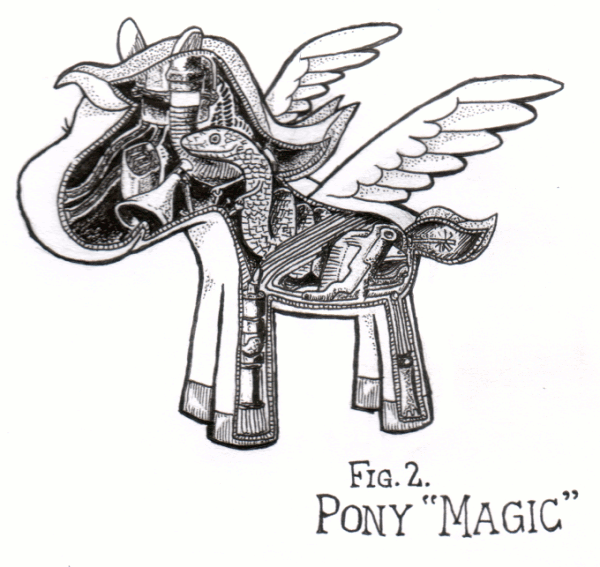
\includegraphics[height=10cm]{pony-magic}
    \end{center}

\end{slide}


\begin{slide}

    \textcolor{blue}{\Large{Wrap Django's classes}}

    \begin{itemize}
        \item Wrap around django where sensible, to implement scalability changes at the highest level.
        \item Views, admin, models, querysets, fields, ...
    \end{itemize}

    \begin{lstlisting}
# project/admin.py
class ModelAdmin(admin.ModelAdmin):
    pass
    \end{lstlisting}

    \begin{lstlisting}
# blog/admin.py
from project.admin import ModelAdmin

class BlogPostAdmin(ModelAdmin):
    # bla bla bla...
    \end{lstlisting}

\end{slide}


\begin{slide}

    \begin{itemize}
        \item e.g. to make all Admin pages use new queryset class (see my \href{http://adamj.eu/tech/2014/07/16/extending-djangos-queryset-to-return-approximate-counts/}{blog post} on approximate counts)
    \end{itemize}

    \begin{lstlisting}
# project/admin.py
class ModelAdmin(admin.ModelAdmin):
    def queryset(self, request):
        qs = super(ModelAdmin, self).queryset(request)
        qs = qs._clone(klass=ApproxCountQuerySet)
        return qs
    \end{lstlisting}

\end{slide}


\begin{slide}

    \textcolor{blue}{\Large{Caching}}

    \begin{center}
        
\includegraphics[height=9cm]{squirrel-eating-nuts}
    \end{center}

    \begin{itemize}
        \item Caches make things faster.
        \item But don't be overzealous - keep your caching/invalidation model simple, and don't use it to sticky tape over more fundamental problems (slow DB, code execution time, ...).
    \end{itemize}

\end{slide}


\begin{slide}

    \begin{itemize}
        \item Monitor all the things (New Relic):
    \end{itemize}

    \begin{center}
        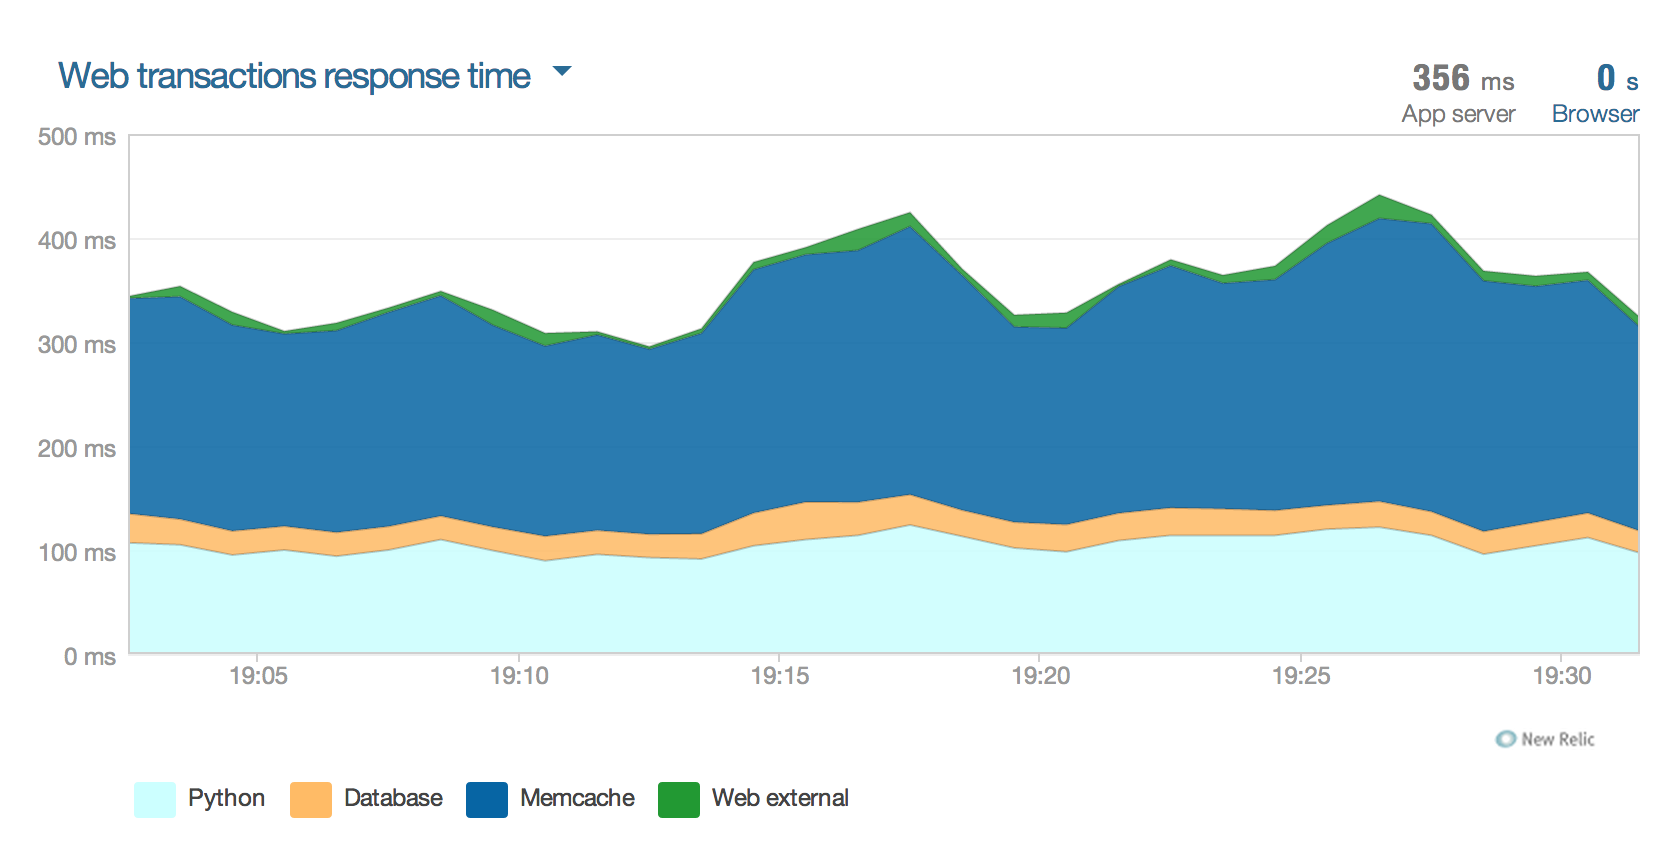
\includegraphics[height=12cm]{web-transactions-1}
    \end{center}

\end{slide}


\begin{slide}

    \begin{itemize}
        \item At scale, percentile view is much more useful:
    \end{itemize}

    \begin{center}
        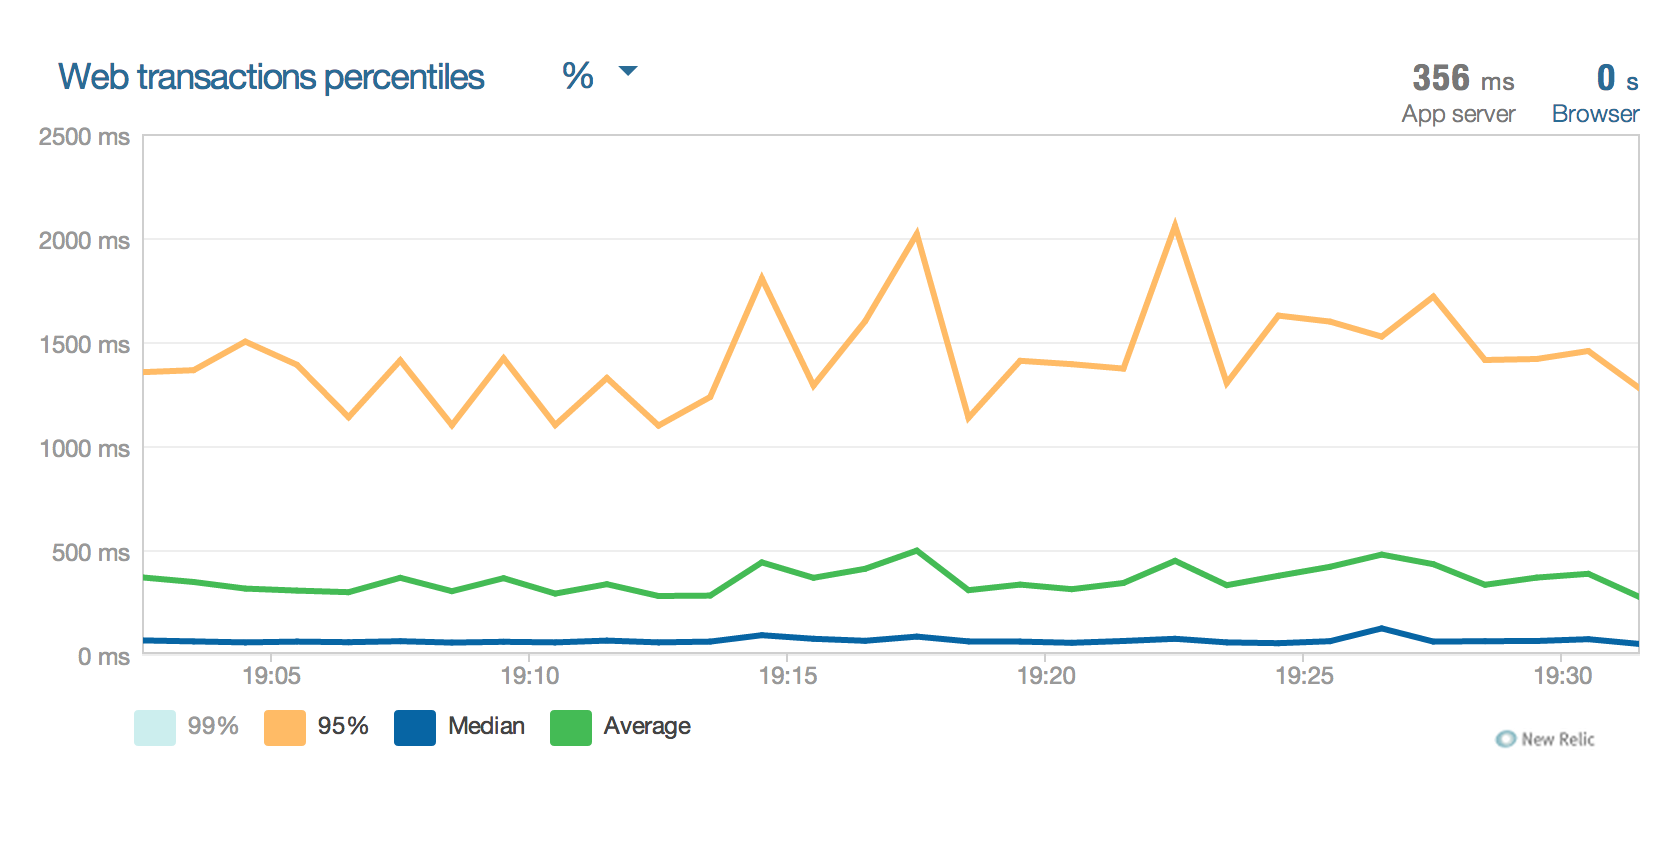
\includegraphics[height=12cm]{web-transactions-2}
    \end{center}

\end{slide}


\begin{slide}

    \textcolor{blue}{\Large{Background fill your cache}}

    \begin{itemize}
        \item Typical cache code puts the refill in the request path:
    \end{itemize}

    \begin{lstlisting}
def some_func(user_id):
    cache_key = 'key:' + str(user_id)
    val = cache.get(cache_key)
    if val is None:
        val = slow_func()
        cache.set(cache_key, val)
    return val
    \end{lstlisting}

    \begin{itemize}
        \item For the 99th percentile power user, a reasonable but slightly slow function call could become way too slow ($>$100ms).
    \end{itemize}

\end{slide}


\begin{slide}

    \begin{itemize}
        \item Instead, use an always-there cache value with a timestamp:
    \end{itemize}

    \begin{lstlisting}
def some_func():
    cache_key = 'key:' + str(user_id)
    last_update, val = cache.get(cache_key)
    if last_update < now() - timedelta(minutes=15):
        # celery task to refill cache_key
        slow_func.apply_async([user_id])
    return val
    \end{lstlisting}

    \begin{itemize}
        \item In-request code path now just one cache fetch for even the 99th percentile user on a bad day.
        \item (Code simplified - you want to put task in queue just once, and maybe use a persistent cache backend.)
    \end{itemize}

\end{slide}


\begin{slide}

    \textcolor{blue}{\Large{Database}}

    \begin{itemize}
        \item Don't be hasty to get away from the ORM or relational databases.
        \item Instead, learn them better.
        \item Understand how Querysets become SQL, how the DB will handle SQL, and find easy wins on this path.
    \end{itemize}

\end{slide}


\begin{slide}

    \textcolor{blue}{\Large{Use prefetch\_related}}

    \begin{itemize}
        \item \textbf{select\_related} on many models will generate a query with a lot of JOIN clauses.
        \item \textbf{prefetch\_related} will generate many smaller simpler queries - one for each table.
        \item It may be counterintuitive, but using \textbf{prefetch\_related} to do app-level JOINs can be faster and is much more scalable.
        \item Django is really friendly here - it's so easy to switch `select' to `prefetch'!
    \end{itemize}

\end{slide}


\begin{slide}

    \textcolor{blue}{\Large{Learn the way of the index}}

    \begin{itemize}
        \item Indexing is an art that takes time to perfect. Some trial and error.
        \item Number one problem in Django - bunging `index=True' on several fields and expecting all queries to magically speed up.
    \end{itemize}

    \begin{center}
        
\includegraphics[height=9cm]{buddhist-monk}
    \end{center}

\end{slide}


\begin{slide}

    \textcolor{blue}{\Large{Run a query killer/sniper}}

    \begin{center}
        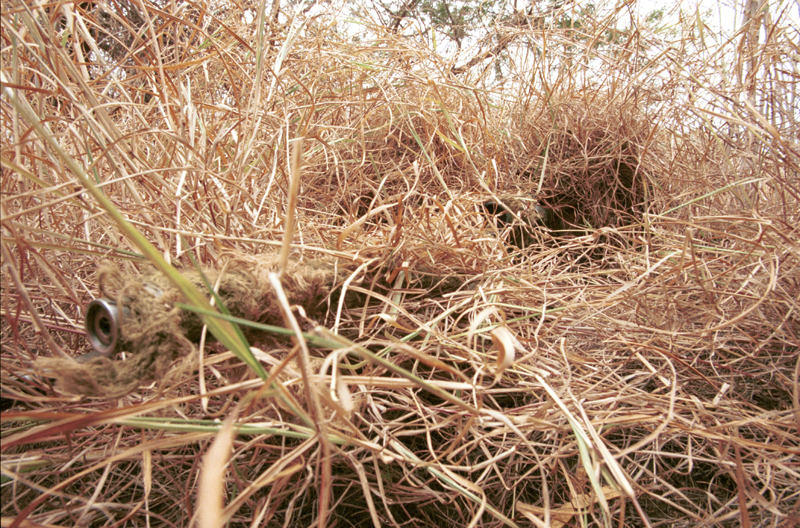
\includegraphics[height=10cm]{Camouflaged-sniper}
    \end{center}

    \begin{itemize}
        \item Web request timed out != query cancelled
        \item Every 10 seconds, kill any query lasting longer than 30 seconds, and email you about it
    \end{itemize}

\end{slide}


\begin{slide}

    \textcolor{blue}{\Large{Use replicas smartly}}

    \begin{center}
        
\includegraphics[height=12cm]{Marian_and_Vivian_Brown}
    \end{center}

    \begin{itemize}
        \item Replicas are amazing, use them.
    \end{itemize}

\end{slide}


\begin{slide}

    \begin{itemize}
        \item You can use a \textbf{DBRouter} in your Django settings to add logic for which DB is used.
        \item Or, you can manually direct certain queries that you know can handle slightly stale data, e.g.:
    \end{itemize}

    \begin{lstlisting}
# project/admin.py
class ModelAdmin(admin.ModelAdmin):
    def queryset(self, request):
        qs = super(ModelAdmin, self).queryset(request)
        if request.method == 'GET':
            qs = qs.using('replica')
        return qs
    \end{lstlisting}

    \begin{itemize}
        \item Routing admin to replica is actually a really big win - stop the big nasty admin queries from affecting the performance of the main app.
    \end{itemize}

\end{slide}


\begin{slide}
    \textcolor{blue}{\Large{Thank you}}

    \begin{itemize}
        \item \url{me@adamj.eu}
    \end{itemize}

\end{slide}

\end{document}
